%hier jede Aufgabe als eigene Datei mit dem Input-Befehl einfügen
%\subsection{Gleichstrommaschine 1\label{AufgGM1}}
\Aufgabe{
    Eine fremderregte Gleichstrommaschine hat die folgenden Angaben auf ihrem Typenschild:
    \begin{itemize}
        \item Nennleistung: $41,8\,\text{kW}$
        \item Nenndrehzahl: $1900\,\frac{1}{\text{min}}$
        \item Ankernennspannung: $440\,\text{V}$
        \item Ankernennstrom: $100\,\text{A}$
        \item Erregung: $240\,\text{V}$
        \item Erregerstrom: $10\,\text{A}$
        \item Leerlaufdrehzahl: $2000\,\frac{1}{\text{min}}$
    \end{itemize}

    Hinweis: Die Nennleistung auf einem Motortypenschild bezeichnet immer die abgegebene mechanische Leistung im Nennpunkt.

    \begin{itemize}
        \item[a)]
        Wie groß ist das Drehmoment der Maschine im Nennpunkt?
        \item[b)]
        Berechnen Sie den Wirkungsgrad der Maschine im Nennpunkt.
        \item[c)]
        Berechnen Sie das Produkt aus Erregerfluss und der Ankerkonstanten $K\cdot \Phi$
        \item[d)]
        Wie groß ist der Ankerwiderstand $R_A$?
    \end{itemize}
}

\Loesung{
	\begin{itemize}

		\item[a)]
		Aus der Nennleistung und der Nenndrehzahl ergibt sich direkt das Nenndrehmoment:
		\begin{align*}
		    P_\text{mech} &= M\cdot \omega\\
		    M &= \frac{P_\text{mech}}{\omega} = \frac{41,8\,\text{kW}}{2\pi\cdot 1900\,\frac{1}{\text{min}} \cdot \frac{1\,\text{min}}{60\,\text{s}}} = 210,08\,\text{Nm}
		\end{align*}
		\item[b)]
		Im Motorbetrieb ist der Wirkungsgrad der Quotient aus mechanischer bezogen auf die elektrische Leistung (siehe Gleichung \ref{GlLeistung}). Hierbei muss sowohl die Ankerleistung, als auch die Erregerleistung berücksichtigt werden.
		\begin{eqa}
			\eta &= \frac{P_\text{mech}}{P_\text{elektr}} = \frac{41,8\,\text{kW}}{440\,\text{V}\cdot 100\,\text{A} + 240\,\text{V}\cdot 10\,\text{A}} = 90,08\,\%\nonumber
		\end{eqa}

		\item[c)]
		Nach Gleichung \ref{GlInduzierteSpannungGM} wird die induzierte Spannung berechnet. Im Leerlauf muss die induzierte Spannung der Ankerspannung entsprechen. Gleiches geht aus Gleichung \ref{GlfremderregteGM1} hervor, da im Leerlauf auch das Drehmoment Null sein muss.
		\begin{eqa}
			U_q &= K \cdot \Phi \cdot \omega\tag{\ref{GlInduzierteSpannungGM}}\\
			K\cdot \Phi &= \frac{U_q}{\omega} = \frac{440\,\text{V}}{2\pi\cdot 2000\,\frac{1}{\text{min}} \cdot \frac{1\,\text{min}}{60\,\text{s}}} = 2,1\,\text{Vs}\nonumber
		\end{eqa}
		\item[d)]
		Hier sind zwei Ansätze möglich. Es kann Gleichung \ref{GlfremderregteGM1} auf den Ankerwiderstand umgeformt werden:
		\begin{eqa}
			n &= \frac{U_A}{2\pi K\cdot \Phi} - \frac{R_A\cdot M_i}{2\pi(K\cdot \Phi)^2}\tag{\ref{GlfremderregteGM1}}\\
			R_A &= \left(\frac{U_A}{2\pi K\cdot \Phi} - n\right) \cdot \frac{2\pi(K\cdot \Phi)^2}{M_i}\nonumber\\
			&= \left(\frac{440\,\text{V}}{2\pi\cdot 2,1\,\text{Vs}} - \frac{1900}{60\,\text{s}}\right)\cdot \frac{2\pi\cdot (2,1\,\text{Vs})^2}{210,08\,\text{Nm}} = 220\,\text{m}\Omega\nonumber
		\end{eqa}
		Die andere Berechnungsvariante führt über das Ersatzschaltbild in Abbildung \ref{AbbGMFremderregt}. Im Nennbetrieb können wir die Quellenspannung $U_q$ berechnen. Diese muss kleiner als die Quellenspannung im Leerlauf sein.
		\begin{eqa}
			U_q &= K \cdot \Phi \cdot \omega \tag{\ref{GlInduzierteSpannungGM}}\\
			U_{q,n}&=  2,1\,\text{Vs} \cdot 2\pi\cdot 1900\,\frac{1}{\text{min}} \cdot \frac{1\,\text{min}}{60\,\text{s}} = 418\,\text{V}\nonumber
		\end{eqa}
		Der Spannungsabfall am Widerstand $R_A$ muss durch dem Maschenumlauf die Differenzspannung zwischen Ankerspannung und induzierter Spannung betragen. Da der Ankerstrom im Nennbetrieb bekannt ist, kann der Widerstand über das Ohmsche Gesetz berechnet werden.
		\begin{equation*}
		    R_A = \frac{U_A - U_q}{I_A} = \frac{440\,\text{V} - 418\,\text{V}}{100\,\text{A}} = 220\,\text{m}\Omega
		\end{equation*}
	\end{itemize}
}
%\input{Aufgabe2}
%....

%Das ist nur Beispielsinhalt, bitte auskommentieren!
%\subsection{Gleichstrommaschine 1\label{AufgGM1}}
\Aufgabe{
    Eine fremderregte Gleichstrommaschine hat die folgenden Angaben auf ihrem Typenschild:
    \begin{itemize}
        \item Nennleistung: $41,8\,\text{kW}$
        \item Nenndrehzahl: $1900\,\frac{1}{\text{min}}$
        \item Ankernennspannung: $440\,\text{V}$
        \item Ankernennstrom: $100\,\text{A}$
        \item Erregung: $240\,\text{V}$
        \item Erregerstrom: $10\,\text{A}$
        \item Leerlaufdrehzahl: $2000\,\frac{1}{\text{min}}$
    \end{itemize}

    Hinweis: Die Nennleistung auf einem Motortypenschild bezeichnet immer die abgegebene mechanische Leistung im Nennpunkt.

    \begin{itemize}
        \item[\bf a)]
        Wie groß ist das Drehmoment der Maschine im Nennpunkt?
        \item[\bf b)]
        Berechnen Sie den Wirkungsgrad der Maschine im Nennpunkt.	
        \item[\bf c)]
        Berechnen Sie das Produkt aus Erregerfluss und der Ankerkonstanten $K\cdot \Phi$
        \item[\bf d)]
        Wie groß ist der Ankerwiderstand $R_A$?
    \end{itemize}
}

\Loesung{
	\begin{itemize}
		
		\item[\bf a)]
		Aus der Nennleistung und der Nenndrehzahl ergibt sich direkt das Nenndrehmoment:
		\begin{align*}
		    P_\text{mech} &= M\cdot \omega\\
		    M &= \frac{P_\text{mech}}{\omega} = \frac{41,8\,\text{kW}}{2\pi\cdot 1900\,\frac{1}{\text{min}} \cdot \frac{1\,\text{min}}{60\,\text{s}}} = 210,08\,\text{Nm}
		\end{align*}
		\item[\bf b)]
		Im Motorbetrieb ist der Wirkungsgrad der Quotient aus mechanischer bezogen auf die elektrische Leistung (siehe Gleichung \ref{GlLeistung}). Hierbei muss sowohl die Ankerleistung, als auch die Erregerleistung berücksichtigt werden.
		\begin{eqa}
			\eta &= \frac{P_\text{mech}}{P_\text{elektr}} = \frac{41,8\,\text{kW}}{440\,\text{V}\cdot 100\,\text{A} + 240\,\text{V}\cdot 10\,\text{A}} = 90,08\,\%\nonumber
		\end{eqa}
		
		\item[\bf c)]
		Nach Gleichung \ref{GlInduzierteSpannungGM} wird die induzierte Spannung berechnet. Im Leerlauf muss die induzierte Spannung der Ankerspannung entsprechen. Gleiches geht aus Gleichung \ref{GlfremderregteGM1} hervor, da im Leerlauf auch das Drehmoment Null sein muss.
		\begin{eqa}
			U_q &= K \cdot \Phi \cdot \omega\tag{\ref{GlInduzierteSpannungGM}}\\
			K\cdot \Phi &= \frac{U_q}{\omega} = \frac{440\,\text{V}}{2\pi\cdot 2000\,\frac{1}{\text{min}} \cdot \frac{1\,\text{min}}{60\,\text{s}}} = 2,1\,\text{Vs}\nonumber
		\end{eqa}
		\item[\bf d)]
		Hier sind zwei Ansätze möglich. Es kann Gleichung \ref{GlfremderregteGM1} auf den Ankerwiderstand umgeformt werden:
		\begin{eqa}
			n &= \frac{U_A}{2\pi K\cdot \Phi} - \frac{R_A\cdot M_i}{2\pi(K\cdot \Phi)^2}\tag{\ref{GlfremderregteGM1}}\\
			R_A &= \left(\frac{U_A}{2\pi K\cdot \Phi} - n\right) \cdot \frac{2\pi(K\cdot \Phi)^2}{M_i}\nonumber\\
			&= \left(\frac{440\,\text{V}}{2\pi\cdot 2,1\,\text{Vs}} - \frac{1900}{60\,\text{s}}\right)\cdot \frac{2\pi\cdot (2,1\,\text{Vs})^2}{210,08\,\text{Nm}} = 220\,\text{m}\Omega\nonumber
		\end{eqa}
		Die andere Berechnungsvariante führt über das Ersatzschaltbild in Abbildung \ref{AbbGMFremderregt}. Im Nennbetrieb können wir die Quellenspannung $U_q$ berechnen. Diese muss kleiner als die Quellenspannung im Leerlauf sein.
		\begin{eqa}
			U_q &= K \cdot \Phi \cdot \omega \tag{\ref{GlInduzierteSpannungGM}}\\
			U_{q,n}&=  2,1\,\text{Vs} \cdot 2\pi\cdot 1900\,\frac{1}{\text{min}} \cdot \frac{1\,\text{min}}{60\,\text{s}} = 418\,\text{V}\nonumber
		\end{eqa}
		Der Spannungsabfall am Widerstand $R_A$ muss durch dem Maschenumlauf die Differenzspannung zwischen Ankerspannung und induzierter Spannung betragen. Da der Ankerstrom im Nennbetrieb bekannt ist, kann der Widerstand über das Ohmsche Gesetz berechnet werden.
		\begin{equation*}
		    R_A = \frac{U_A - U_q}{I_A} = \frac{440\,\text{V} - 418\,\text{V}}{100\,\text{A}} = 220\,\text{m}\Omega
		\end{equation*}
	\end{itemize}
}
\subsection{Komplexe Zahlen 1}
\Aufgabe{
    Es gelte für folgende komplexe Zahlen: \\
    $Z_1 = 3+j4$  \\
    $Z_2 = 2-j$   \\
    $Z_3 = j7$    \\

    Berechnet werden sollen folgende Aufgabenteile:
    \begin{itemize}
        \item [\bf a)] $Z_1 + Z_2$
        \item [\bf b)] $Z_1 - Z_3$
        \item [\bf c)] Polarform von $Z_1$, $Z_2$ und $Z_3$
        \item [\bf d)] $Z_1 \cdot Z_2$
        \item [\bf e)] $\frac{Z_1}{Z_3}$
        \item [\bf f)] Zeigerdiagramm von $Z_1 + Z_2$ und $Z_1 \cdot Z_2$
    \end{itemize}
}


\Loesung{
	\begin{itemize}

	\item[\bf a)]   $Z_1 + Z_2$\\
    \begin{eqa}
        Z_1 + Z_2 &= (3 + j4) + (2 - j) \nonumber   \\
        &= 5 + j3   \nonumber   
    \end{eqa}


    \item[\bf b)] $Z_1 - Z_3$\\\\
    
    \begin{eqa}
        Z_1 - Z_3 &= (3 + j4) - (0 + j7)    \nonumber   \\ 
        &= 3 - j3   \nonumber   
    \end{eqa}

    \item[\bf c)] Polarform von $ Z_1, Z_2$ und $Z_3 $\\
    
    \begin{eqa}
        Z_1 &= 5 \cdot \mathrm{e}^{\mathrm{j}53.13^\circ}  \nonumber  \\
        Z_2 &= 2,236 \cdot \mathrm{e}^{\mathrm{j}-26,57^\circ}  \nonumber \\
        Z_3 &= 7 \cdot \mathrm{e}^{\mathrm{j}90^\circ}   \nonumber 
    \end{eqa}
    

    \item[\bf d)] $Z_1 \cdot Z_2$\\
    
    \begin{eqa}
        Z_1 \cdot Z_2 &= (3 + j4) \cdot (2 - j) \nonumber   \\
        &= 10 + j5  \nonumber
    \end{eqa}


    \item[\bf e)] $\frac{Z_1}{Z_3} $\\
    
    \begin{eqa}
        \frac{Z_1}{Z_3} = \frac{3 + j4}{j7} \nonumber
    \end{eqa}

    (Erweitern mit dem konjugierten Wert des Nenners, also -j7)\\

    \begin{eqa}
        \frac{3 + j4}{j7} \cdot \frac{-j7}{-j7} = \frac{(3 + j4) \cdot (-j7)}{(j7) \cdot (-j7)}     \nonumber
    \end{eqa}

    Hinweis: $j^2 = -1$\\

    \begin{eqa}
        \frac{Z_1}{Z_3} &= \frac{28 - j21}{49} = \frac{28}{49} - j \frac{21}{49} = \frac{4}{7} - j \frac{3}{7}  \nonumber   \\
        &= \frac{4}{7} - j \frac{3}{7}    \nonumber
    \end{eqa}
    

\newpage
    
    \item[\bf f)] Zeigerdiagramm von $Z_1 + Z_2 $ und $Z_1 \cdot Z_2 $
    
    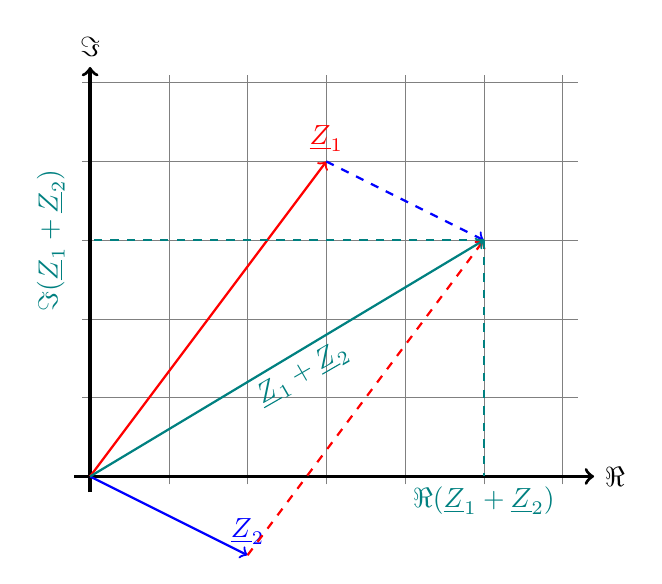
\begin{tikzpicture}
        \draw (0,0) coordinate (K);
        \draw[very thin,gray] (-0.1,-0.1) grid (6.2,5.1);
        \draw[->, very thick] (-0.2,0) -- (6.4,0) node[right] {$\Re$};
        \draw[->, very thick] (0,-0.2) -- (0,5.2) node[above] {$\Im$};
        \draw[->, thick, red] (0,0) -- (3,4) node[above] {$\underline{Z}_\mathrm{1}$};
        \draw[->, thick, blue] (0,0) -- (2,-1) node[above] {$\underline{Z}_\mathrm{2}$};
        
       
        \draw[->, dashed, thick, blue] (3,4) -- (5,3) ;
        \draw[->, dashed, thick, red] (2,-1) -- (5,3) ; 
        
       
        \draw[->, thick, teal] (0,0) -- (5,3);
        \draw(2.7,1.3) node [teal, rotate=30] {$\underline{Z}_\mathrm{1}+\underline{Z}_\mathrm{2}$};
        \draw[dashed, thick, teal] (5,3) -- (0,3)
        (-0.5,3) node[rotate=90] {$\Im(\underline{Z}_\mathrm{1}+\underline{Z}_\mathrm{2}$)};
        \draw[dashed, thick, teal] (5,3) -- (5,0) node[below] {$\Re(\underline{Z}_\mathrm{1}+\underline{Z}_\mathrm{2}$)};
    \end{tikzpicture}\\
    %{{\bf Addition von komplexen Zahlen.} Zeichnerische Lösung einer Addition von zwei komplexen Zahlen im Zeigerdiagramm}\\


    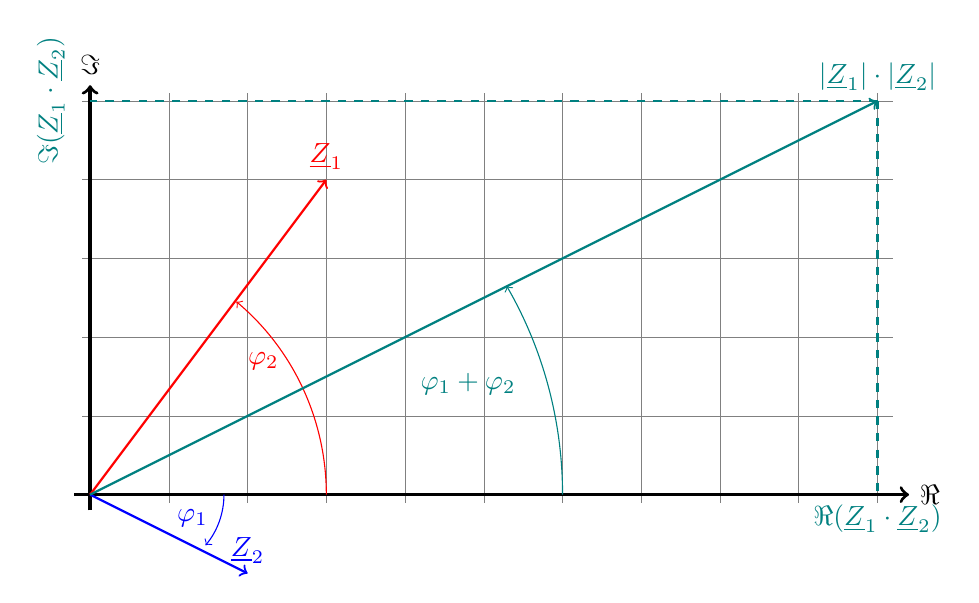
\begin{tikzpicture}
        \draw (0,0) coordinate (K);
        \draw[very thin,gray] (-0.1,-0.1) grid (10.2,5.1);
        \draw[->, very thick] (-0.2,0) -- (10.4,0) node[right] {$\Re$};
        \draw[->, very thick] (0,-0.2) -- (0,5.2) node[above] {$\Im$};

        \draw[->, thick, red] (0,0) -- (3,4) node[above] {$\underline{Z}_\mathrm{1}$};
        \draw[->, thick, blue] (0,0) -- (2,-1) node[above] {$\underline{Z}_\mathrm{2}$};
        \draw [->,blue] (1.7,0) arc (0:-40:1cm);
    \draw [->,red] (3,0) arc (0:50:3.2cm);
    \draw [->,teal] (6,0) arc (0:30:5.3cm);
        \draw[->, thick, teal] (0,0) -- (10,5) node [above] {$|\underline{Z}_\mathrm{1}| \cdot |\underline{Z}_\mathrm{2}|$};
    % {{\bf Multiplikation von komplexen Zahlen.} Zeichnerische Lösung einer Multiplikation von zwei komplexen Zahlen im Zeigerdiagramm}
    \draw[dashed, thick, teal] (10,5) -- (10,0) node[below] {$\Re(\underline{Z}_\mathrm{1} \cdot \underline{Z}_\mathrm{2}$)};
    \draw[dashed, thick, teal] (10,5) -- (0,5)
    (-0.5,5) node[rotate=90] {$\Im(\underline{Z}_\mathrm{1} \cdot \underline{Z}_\mathrm{2}$)};
    \node [red] at (2.2,1.7) {$\varphi_\mathrm{2}$};
    \node [blue] at (1.3,-0.3) {$\varphi_\mathrm{1}$};
    
    \node [teal] at (4.8,1.4) {$\varphi_\mathrm{1} + \varphi_\mathrm{2}$};
    \end{tikzpicture}\\
	


\end{itemize}

}
\subsection{Komplexe Zahlen 2}
\Aufgabe{
    Es gelte für folgende komplexe Zahlen: \\
    $K_1 = 10 + j40$  \\
    $K_2 = 50 \cdot e^{-j40^o}$   \\
    $K_3 = 250 \cdot e^{j\frac{\pi}{4}}$    \\

    Berechnet werden sollen folgende Aufgabenteile:
    \begin{itemize}
        \item [\bf a)] $K_1 - K_2$, Ergebnis in Polarkoordinaten
        \item [\bf b)] $K_3 + K_2$, Ergebnis in kartesischen Koordinaten
        \item [\bf c)] $K_1 \cdot K_3$, Ergebnis in Polarkoordinaten 
        \item [\bf d)] $K_1 + K_2$, zeichnerisch im Zeigerdiagramm
        \item [\bf e)] $(K_1 - K_2)^2$
        \item [\bf f)] $\sqrt{K_1 + K_3}$
    \end{itemize}
}


\Loesung{
	\begin{itemize}

	\item[\bf a)]   $K_1 - K_2$, Ergebnis in Polarkoordinaten
    
    \begin{eqa}
        10 + \mathrm{j} \cdot 40 - 50 \cdot \mathrm{e}^{-\mathrm{j}40^\circ} = ? \nonumber 
    \end{eqa}
    
    $\underline{K}_2$ in kartesische Koordinaten wandeln: 

    \begin{eqa}
        50 \cdot \mathrm{e}^{-\mathrm{j}40^\circ} &= 50 \cdot \cos(-40^\circ) + \mathrm{j} 50 \cdot \sin(-40^\circ)  \nonumber   \\
        &= 50 \cdot 0,766 + \mathrm{j} 50 \cdot (-0,6427)  \nonumber   \\
        &= 38,302 - \mathrm{j} 32,1393  \nonumber
    \end{eqa}
    
    $\underline{K}_2 - \underline{K}_2$ in kartesischen Koordinaten subtrahieren: 

    \begin{eqa}
        \underline{K}_1 - \underline{K}_2 &= (10 + \mathrm{j} \cdot 40) - (38,302 - \mathrm{j} 32,1393) \nonumber   \\
        &= 10 + \mathrm{j} \cdot 40 - 38,302 + \mathrm{j} 32,1393 \nonumber   \\
        &= -28,3 + \mathrm{j} 72,139    \nonumber
    \end{eqa}

    Ergebnis in Polarkoordinaten: 

    \begin{eqa}
        \underline{K}_1 - \underline{K}_2 &= \sqrt{\Re^2+\Im^2} \cdot \mathrm{e}^{\mathrm{j}\arctan(\frac{\Im}{\Re})} \nonumber   \\
        &= 77,49 \cdot \mathrm{e}^{\mathrm{j}111,42^\circ}  \nonumber
    \end{eqa}

    \item[\bf b)] $K_3 + K_2$, Ergebnis in kartesischen Koordinaten
    
    \begin{eqa}
        K_3 &= 250 \cdot e^{j\frac{\pi}{4}} = 176,78 + j176,78  \nonumber   \\
        K_2 &= 50 \cdot e^{-j40^\circ} = 38,3 - j32,15  \nonumber   \\
        K_3 + K_2 &= (176,78 + j176,78) + (38,3 - j32,15)  \nonumber   \\
        K_3 + K_2 &= 215,08 + j144,63  \nonumber   
    \end{eqa}

    \item[\bf c)] $K_1 \cdot K_3$, Ergebnis in Polarkoordinaten

    \begin{eqa}
        \underline{K}_1 &= 10 + \mathrm{j}40   \nonumber   \\
        &= 41,23 \cdot \mathrm{e}^{\mathrm{j}75,96^\circ}  \nonumber  \\
        \underline{K}_1 \cdot \underline{K}_3 &= 10 + \mathrm{j}40  \cdot 250 \cdot \mathrm{e}^{\mathrm{j}45^\circ}    \nonumber   \\
        &= 10307,75 \cdot \mathrm{e}^{\mathrm{j}120,96^\circ}  \nonumber  
    \end{eqa}

    \item[\bf d)] $K_1 + K_2$, zeichnerisch im Zeigerdiagramm
    
    \begin{figure}[H]
        \centering
        \resizebox{0.3\textwidth}{!}{
            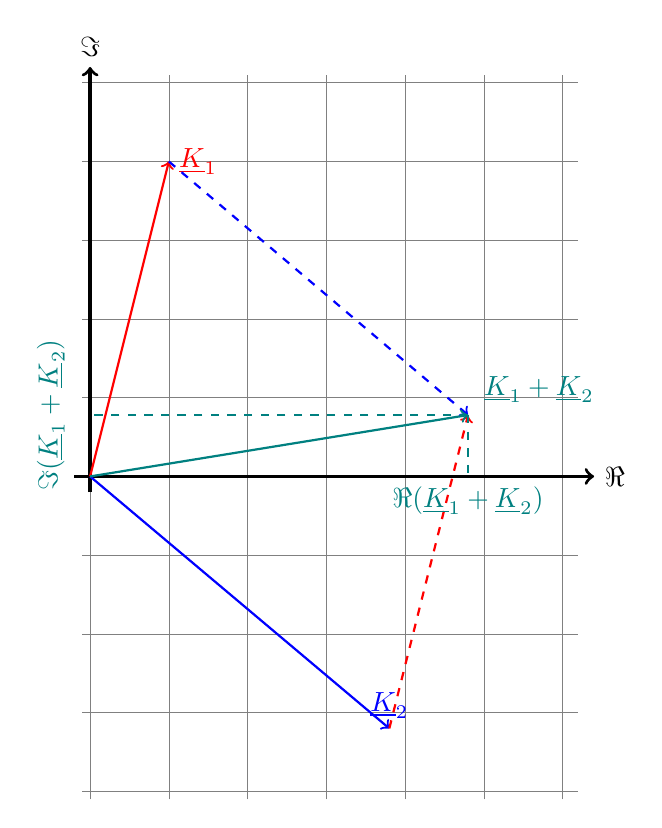
\begin{tikzpicture}
                \draw (0,0) coordinate (K);
                \draw[very thin,gray] (-0.1,-4.1) grid (6.2,5.1);
                \draw[->, very thick] (-0.2,0) -- (6.4,0) node[right] {$\Re$};
                \draw[->, very thick] (0,-0.2) -- (0,5.2) node[above] {$\Im$};
                \draw[->, thick, red] (0,0) -- (1,4) node[right] {$\underline{K}_\mathrm{1}$};
                \draw[->, thick, blue] (0,0) -- (3.8,-3.2) node[above] {$\underline{K}_\mathrm{2}$};
                
                \draw[->, dashed, thick, blue] (1,4) -- (4.8,0.78);
                \draw[->, dashed, thick, red] (3.8,-3.2) -- (4.8,0.78);
                
            
                \draw[->, thick, teal] (0,0) -- (4.8,0.78);
                \draw(5.7,1.1) node [teal] {$\underline{K}_\mathrm{1}+\underline{K}_\mathrm{2}$};
                \draw[dashed, thick, teal] (4.8,0.78) -- (0,0.78)
                (-0.5,0.78) node[rotate=90] {$\Im(\underline{K}_\mathrm{1}+\underline{K}_\mathrm{2}$)};
                \draw[dashed, thick, teal] (4.8,0.78) -- (4.8,0) node[below] {$\Re(\underline{K}_\mathrm{1}+\underline{K}_\mathrm{2}$)};
            \end{tikzpicture}
        }
    \end{figure}

    \item[\bf e)] $(K_1 - K_2)^2$
    
    Ergebnis aus Teil a): 
    \begin{eqa}
        K_1 - Z_2 = 77,49 \cdot \mathrm{e}^{\mathrm{j}111,42^\circ} \nonumber  
    \end{eqa}
    
    Regel für das Quadrat einer komplexen Zahl:
    \begin{eqa}
        (K_1 - K_2)^2 &= 77,49^2 \cdot \mathrm{e}^{\mathrm{j}2 \cdot 111,42^\circ}    \nonumber   \\
        &= 6004 \cdot \mathrm{e}^{-\mathrm{j}137^\circ} \nonumber 
    \end{eqa} 
    

    \item[\bf f)] $\sqrt{K_1 + K_3}$
    
    \begin{eqa}
        K_1 + K_3 = 186,78 + j216,78    \nonumber   
    \end{eqa}
    
    Umwandlung in Polarform:

    \begin{eqa}
        K_1 + K_3 = 286,09 \cdot \mathrm{e}^{\mathrm{j}49,32^\circ}   \nonumber   
    \end{eqa}
    
    Die Quadratwurzel einer komplexen Zahl in Polarform ergibt:

    \begin{eqa}
        \sqrt{r \cdot \mathrm{e}^{\mathrm{j}\varphi}} &= \sqrt{r} \frac{\varphi}{2}  \nonumber   \\
        \sqrt{286,09} \cdot \mathrm{e}^{\mathrm{j}\frac{49,32^\circ}{2}} &= 16,91 \cdot \mathrm{e}^{\mathrm{j}24,66^\circ}  \nonumber
    \end{eqa}

\end{itemize}

}
\subsection{Zeigerdiagramme 1}
\Aufgabe{
    
    Gegeben sei die Spannung $\hat{U} = 325\ V \cdot \mathrm{e}^{\mathrm{j}30^\circ}$.

    \begin{itemize}
        \item [\bf a)] Zeichnen Sie das Zeigerdiagramm für die Spannung $\hat{U}$ im komplexen Zahlenraum.
        \item [\bf b)] Berechnen Sie die Real- und Imaginärteile der komplexen Spannung $\hat{U}$.
        \item [\bf c)] Erklären Sie die Bedeutung des Phasenwinkels in Bezug auf die Wechselspannung.
    \end{itemize}
}

\Loesung{
	\begin{itemize}

	\item[\bf a)]
	Zeigerdiagramm für die Spannung $\hat{U}$ \\

    \begin{figure}[H]
        \centering
        \resizebox{0.3\textwidth}{!}{
        \begin{tikzpicture}
            % Achsen zeichnen
            \draw[->] (-0.5,0) -- (3,0) node[right] {$\Re$};
            \draw[->] (0,-0.5) -- (0,1.5) node[above] {$\Im$};
        
            % Zeiger zeichnen
            \draw[->, thick, color=voltage] (0,0) -- ({2 * cos(30)},{2 * sin(30)}) node[above right] {$\hat{U}$};
        
            % Winkel markieren
            \draw[->] (0,0) -- (0.5,0) node[below] {$0^\circ$};
        
            % Beschriftung
            \node at (2,0.8) {$30^\circ$};
        \end{tikzpicture}
        } 
    \end{figure} 

	\item[\bf b)] 
        Die Real- und Imaginärteile der Spannung $\hat{U}$ können mit den folgenden Formeln berechnet werden:

        \begin{eqa}
            U_{\text{Re}} &= \hat{U} \cdot \cos(\varphi) = 325 \cdot \cos(30^\circ) \approx 281,46\ V      \nonumber   \\
            U_{\text{Im}} &= \hat{U} \cdot \sin(\varphi) = 325 \cdot \sin(30^\circ) = 162,5\ V   \nonumber
        \end{eqa}

	\item[\bf c)] 
    Der Phasenwinkel $\varphi$ beschreibt den zeitlichen Versatz zwischen der Spannung und dem Strom in einem Wechselstromkreis. 
    Ein positiver Phasenwinkel deutet darauf hin, dass die Spannung der Strom nachfolgt (induktive Last), während ein negativer 
    Phasenwinkel anzeigt, dass der Strom der Spannung nachfolgt (kapazitive Last). 

\end{itemize}

}
\subsection{Komplexe Wechselstromrechnung 1}
\Aufgabe{
    Gegeben sind die spezifischen Werte für den Widerstand $R$, die Spule $L$ und den Kondensator $C$. \\
    $R=10\ \Omega$, $L=10\ mH$, $C=10\ pF$
    \\
    Berechnet werden sollen die Impedanzen der drei Bauteile bei den Frequenzen:\\
    $1\ \mu Hz$,$1\ mHz$,$1\ Hz$,$1\ kHz$,$1\ MHz$ \\
    \\
    Tragen Sie die Ergebnisse in eine Tabelle ein.
}


\Loesung{
	\begin{itemize}

	\item[] 
	\begin{table}[H]
        \centering
            \begin{tabular}{  c  c  c  c }
                \hline
                ${\bf Frequenz}$ & ${\bf X_R}$ & ${\bf X_C}$ & ${\bf X_L}$ \\
                \hline
                $1\ \mu Hz$ & $10\ \Omega$ & $-j 15,92\ M\Omega$ & $j 6,28$ \\
                $1\ mHz$ & $10\ \Omega$ & $-j 15,92\ k\Omega$ & k \\
                $1\ Hz$ & $10\ \Omega$  & $-j 15,92\ \Omega$ & k \\
                $1\ kHz$ & $10\ \Omega$ & $-j 15,92\ m\Omega$ & \\
                $1\ MHz$ & $10\ \Omega$ & $-j 15,92\ \mu \Omega$ & \\
                \hline
            \end{tabular}
    \end{table}

    

\end{itemize}

}
\subsection{Komplexe Wechselstromrechnung 2}
\Aufgabe{

    Eine Impedanz weist bei der Frequenz $f = 1\ kHz$ den Wert $\underline{Z} = (300+\mathrm{j}400)\ \Omega$ auf. 
    
    \begin{itemize}
        \item[\bf a)] Bestimmen Sie den Scheinwiderstand (Betrag) der Impedanz.
        \item[\bf b)] Ermitteln Sie die Admittanz $\underline{Y} = \frac{1}{\underline{Z}}$ sowie den Scheinleitwert.
        \item[\bf c)] Geben Sie zur Realisierung der Impedanz $\underline{Z}$ eine Schaltung aus zwei in Reihe geschalteten
              Bauelementen an und dimensionieren Sie diese Schaltung.
        \item[\bf d)] Geben Sie zur Realisierung der Impedanz $\underline{Z}$ eine Schaltung aus zwei parallel geschalteten
              Bauelementen an und dimensionieren Sie diese Schaltung.  
    \end{itemize}
    
    Außerdem wird an die Impedanz $\underline{Z} = (300+\mathrm{j}400)\ \Omega$ eine Spannung 
    $u(t)=\hat{U} \cdot \cos(2\pi f t + \varphi_U)$ mit $\hat{U}=5\ V$, $\varphi_U=\pi/4$ und $f=1\ kHz$ gelegt. 
    
    \begin{itemize}
        \item[\bf e)] Ermitteln Sie die komplexe Amplitude $\underline{\hat{U}}$ der anliegenden Spannung.
        \item[\bf f)] Berechnen Sie die komplexe Amplitude $\underline{\hat{I}}$ des Stromes durch die Impedanz.
        \item[\bf g)] Geben Sie den zeitlichen Verlauf des Stromes $i(t)$ an.
        \item[\bf h)] Stellen Sie die Impedanz in Polarform dar und geben Sie den Winkel $\varphi = arg\{\underline{Z}\}$
              an. Vergleichen Sie den Winkel der Impedanz mit der Phasenverschiebung zwischen Spannung und Strom. Was stellen
              Sie fest? 
    \end{itemize}
}


\Loesung{
    \begin{itemize}

        \item[\bf a)]
              \begin{eqa}
                  |\underline{Z}| &= \sqrt{Re^2+Im^2} \nonumber \\  
                  &= \sqrt{300^2+400^2}\ \Omega \nonumber \\ 
                  &= 500\ \Omega     \nonumber
              \end{eqa}
              
        \item[\bf b)]
              \begin{eqa}
                  \underline{Y} &= \frac{1}{\underline{Z}} = \frac{1}{(300+\mathrm{j}400)\ \Omega} \nonumber \\  
                  &= \frac{1}{(300+\mathrm{j}400)\ \Omega} \cdot \frac{(300-\mathrm{j}400)\ \cancel{\Omega}}{(300-\mathrm{j}400)\ \cancel{\Omega}} \nonumber \\ 
                  &= \frac{1}{300^2+400^2} \cdot (300-\mathrm{j}400)\ S     \nonumber   \\
                  &= (0.0012-\mathrm{j}0.0016)\ S     \nonumber     \\
                  |\underline{Y}| &= \frac{1}{|\underline{Z}|} \nonumber      \\
                  &= \frac{1}{500}\ S     \nonumber
              \end{eqa}
              
        \item[\bf c)] 
              Reihenschaltung: \\
              Realteil $\rightarrow$ Ohmscher Wiederstand \\
              Imaginärteil $\rightarrow$ Spule oder Kondensator? \\
              Reaktanz Spule: $X_L=2\pi f \cdot L > 0$       \\
              Reaktanz Kondensator: $X_C=-\frac{1}{2\pi f\cdot C}  < 0$   \\
              
              \begin{figure}[H]
                  \centering
                  \resizebox{0.35\textwidth}{!}{
                      \begin{circuitikz}
    \draw(0,0) to [R=${R}$, o-] (2,0);
    \draw(2,0) to [L=${L}$, -o] (4,0);
\end{circuitikz}
                  }
              \end{figure}
              
              \begin{eqa}
                  R &= 300\ \Omega     \nonumber   \\
                  L &= \frac{X_L}{2\pi \cdot f} \nonumber  \\
                  &= \frac{400\ \Omega}{2\pi \cdot 1\ kHz}  \nonumber   \\
                  &= 63.66\ mH  \nonumber   \\
                  \underline{Z} &= R+\mathrm{j}X_L = R+\mathrm{j}\ 2\pi \cdot f \cdot L        \nonumber
              \end{eqa}
              
        \item[\bf d)]
              Parallelschaltung: \\
              $\rightarrow$ Addition von Leitwerten:\\
              
              \begin{eq}
                  \underline{Y} = G + \mathrm{j}B = (0.0012-\mathrm{j}0.0016)\ S    \qquad  (\text{aus b)})      \nonumber
              \end{eq}
              
              $B<0 \rightarrow$   Spule, induktiver Blindleitwert \\
              $B>0 \rightarrow$   Kondensator, kapazitiver Blindleitwert  \\
              
              \begin{figure}[H]
                  \centering
                  \resizebox{0.5\textwidth}{!}{
                      \begin{circuitikz}
    \draw(0,0) to [short,o-*] (2,0);
    \draw(2,-1) to [short] (2,1);
    \draw(2,1) to [R=${R}$] (4,1);
    \draw(2,-1) to [L=${L}$] (4,-1);
    \draw(4,-1) to [short] (4,1);
    \draw(4,0) to [short,*-o] (6,0);
\end{circuitikz}
                  }
              \end{figure}
              
              \begin{eqa}
                  R &= \frac{1}{G}    \nonumber   \\
                  &= \frac{1}{0.0012\ S}    \nonumber   \\
                  &= 833\ \Omega     \nonumber   \\
                  B &= -\frac{1}{2\pi \cdot f \cdot L} \nonumber  \\
                  L &= \frac{1}{2\pi \cdot f \cdot B}  \nonumber   \\
                  &= 99.47\ mH  \nonumber   
              \end{eqa}
              
        \item[\bf e)] 
              \begin{eqa}
                  \underline{U} &= \hat{U} \cdot \mathrm{e}^{\mathrm{j} \varphi_\mathrm{U}}  = 5\ V \cdot \mathrm{e}^{\mathrm{j} \pi/4} = 5\ V \cdot \mathrm{e}^{\mathrm{j} 45^\circ}    \nonumber   \\
                  &= 5\ V \cdot (\cos(45^\circ)+\mathrm{j}\sin(45^\circ))    \nonumber   \\
                  &= 5\ V \cdot \frac{\sqrt{2}}{2} (1+\mathrm{j}) \nonumber   \\
                  &\approx (3,53 + \mathrm{j} 3,53) \ V    \nonumber
              \end{eqa}
              
        \item[\bf f)]
        
        \item[\bf g)] 
        
        \item[\bf h)] 
        
    \end{itemize}
    
}
%\subsection{Komplexe Wechselstromrechnung 3}
\Aufgabe{

    Das nachfolgende elektrische Netzwerk soll als Beispiel eines Ersatzschaltbildes einer Lithium-Ionen Zelle auf seine
    komplexen Größen analysiert werden. Das Ersatzschaltbild besteht aus einer Serienschaltung aus einer Spule $L$, dem 
    Serienwiderstand $R_\mathrm{S}$ und der Paralellschaltung der Paralellwiderstandes $R_\mathrm{P}$ und dem paralell
    verschalteten Kondensator $C_\mathrm{P}$. Die Berechnung der komplex Ströme und Spannungen aller Komponenten soll in 
    der folgenden Reihenfolge stattfinden:
    
    \begin{itemize}
        \item[\bf a)] Größe der komplexen Impedanzen aller Komponenten und der gesamten komplexen Impedanz
        \item[\bf b)] Komplexe Ströme durch die Komponenten
        \item[\bf c)] Komplexe Spannungen an den Komponenten
    \end{itemize}
    
    \begin{figure}[H]
        \centering
        \resizebox{0.7\textwidth}{!}{
            \begin{circuitikz}

    \draw(0,0) to [L=${L=900\ nH}$, v, i, name=L, o-] (3,0);
    \varrmore{L}{$U_\mathrm{L}$};
    \iarrmore{L}{$I_\mathrm{L}$};

    \draw(3,0) to [R=${R_\mathrm{S}=20\ m\Omega}$, v, i, name=Rs, -*] (6,0);
    \varrmore{Rs}{$U_\mathrm{R_\mathrm{S}}$};
    \iarrmore{Rs}{$I_\mathrm{R_\mathrm{S}}$};

    \draw(6,-1) to [short] (6,1);
    \draw(9,-1) to [short] (9,1);
    \draw(9,0) to [short, *-o] (10,0);

    \draw(6,1) to [R=${R_\mathrm{P}=15\ m\Omega}$, v, i, name=Rp] (9,1);
    \varrmore{Rp}{$U_\mathrm{R_\mathrm{P}}$};
    \iarrmore{Rp}{$I_\mathrm{R_\mathrm{P}}$};

    \draw(6,-1) to [C=${C_\mathrm{P}=200\ mF}$, v, i, name=C] (9,-1);
    \varrmore{C}{$U_\mathrm{C_\mathrm{P}}$};
    \iarrmore{C}{$I_\mathrm{C_\mathrm{P}}$};
\end{circuitikz}
        }
    \end{figure}
}


\Loesung{
    \begin{itemize}

        \item[\bf a)]
              \begin{eq}
                  X_\mathrm{L} = j \omega \cdot L = j \cdot 2\pi \cdot 800\ Hz \cdot 900\ nH  \nonumber
              \end{eq}
              \begin{eq}
                  X_\mathrm{Rs} = R_\mathrm{S} = 20\ m\Omega
              \end{eq}
              
        \item[\bf b)]
        
        \item[\bf c)]  
        
    \end{itemize}
    
}
\subsection{Effektivwert 1}
\Aufgabe{

    Gegeben sei eine sinusförmige Spannung
    
    \begin{eq}
        u(t) = 150\ V \cdot \sin(100\pi t)  \nonumber
    \end{eq}

    wobei $t$ in Sekunden und die Spannung $u(t)$ in Volt angegeben sind.\\

    Berechnen Sie für diese Spannung:

    \begin{itemize}
        \item[\bf a)] Den \textbf{arithmetischen Mittelwert} $\bar{u}$ der Spannung über eine Periode.
        \item[\bf b)] Den \textbf{Effektivwert} $U_{Eff}$ der Spannung.
    \end{itemize}
}

\Loesung{
	\begin{itemize}

	\item[\bf a)]
        Der arithmetische Mittelwert einer Funktion u(t) über eine Periode T ist gegeben durch:
        \begin{eq}
            \bar{u} = \frac{1}{T} \int_0^T u(t) dt  \nonumber
        \end{eq}
        
        Da $u(t)$ eine Sinusfunktion darstellt und die Sinuswelle über eine Periode symmetrisch ist, heben 
        sich die positiven und negativen Teile der Welle gegenseitig auf. Daher ist der arithmetische 
        Mittelwert für jede Sinuswelle immer null:
        
        \begin{eq}
            \bar{u} = 0 \nonumber
        \end{eq}

    \item[\bf b)]
        Der Effektivwert einer Sinusspannung $u(t)$ wird durch die folgende Formel berechnet:
        \begin{eq}
            U_{Eff} = \frac{\hat{U}}{\sqrt{2}}   \nonumber
        \end{eq}
        
        In diesem Fall ist $\hat{U} = 150\ V$, die Amplitude der Spannung.
        
        \begin{eq}
            U_{Eff} = \frac{150\ V}{\sqrt{2}} \approx \frac{150\ V}{1.414} \approx 106.1\ V  \nonumber
        \end{eq}
	
\end{itemize}

}
\subsection{Leistungsberechnung 1}
\Aufgabe{

    Text

    \begin{figure}[H]
        \centering
        \resizebox{0.7\textwidth}{!}{
            \begin{circuitikz}[domain=0:8,samples=100]
                %Gitter
                \draw[very thin,color=gray] (-0.1,-2.1) grid (8.2,2.1);
                \draw[->] (-0.2,0) -- (8.5,0) node[right] {t in ms};
                \draw[->] (0,-2.1) -- (0,2.2) node[above] {};
                \draw (0,-2.1) node[below] {$0$};
                \draw (2,-2.1) node[below] {$25$};
                \draw (4,-2.1) node[below] {$50$};		
                \draw (6,-2.1) node[below] {$75$};
                \draw (8,-2.1) node[below] {$100$};								
                \draw[color=blue] (-0.5,1.5) node[] {$u(t)$};					
                \draw[color=red] (-0.5,-1) node[] {$i(t)$};			
                \draw[color=blue,smooth] plot[id=Sinus14] function{1.5 * sin(pi/2 * x)} node[right] {};
                \draw[color=red,smooth] plot[id=Sinus15] function{2 * sin((pi/2) * x - (pi/3))} node[right] {};
            \end{circuitikz}
        } 
    \end{figure} 

    \begin{itemize}
        \item[\bf a)] Ablesen des Betrages der Phasenwinkel von Spannung und Strom. Bennenung des Verhaltens.
        \item[\bf b)] Angabe von Periodendauer, Frequenz und Kreisfrequenz.
        \item[\bf c)] Berechnung der Augenblicksleistung zum Zeitpunkt t = 12,5\ ms.
        \item[\bf d)] Berechnung von Wirkleistung und Blindleistung.
        \item[\bf e)] Berechnung der Scheinleistung mit dem konjugierten komplexen Strom.  
    \end{itemize}

}

\Loesung{
	\begin{itemize}

        \item[\bf a)]
            Die Spannung weist einen Phasenwinkel von $\varphi_\mathrm{u}=0$ und der Strom weist einen Phasenwinkel von $\varphi_\mathrm{i}=\pi/3$ auf. \\
            Das Nacheilen des Stromes deutet auf ein {\bf induktives Verhalten} hin. 
        
        \item[\bf b)]
            Die Periodendauer T beträgt $50\ ms$. \\
            Die Frequenz beträgt:
            \begin{eq}
                f=\frac{1}{T}=\frac{1}{50\ ms}= 20\ Hz   \nonumber
            \end{eq}
            Die Kreisfrequenz beträgt:
            \begin{eq}
                \omega = 2\pi \cdot f = 2\pi \cdot 20\ Hz = 125,66\ Hz  \nonumber
            \end{eq}

        \item[\bf c)]
            Die Augenblicksleistung zum Zeitpunkt t = 12,5\ ms beträgt:
            \begin{eqa}
                p(t) &= u(t) \cdot i(t) = 12\ V \cdot \sin(2\pi\cdot20\ Hz\cdot 0,0125\ s) \cdot 2\ A \cdot \sin(2\pi\cdot20\ Hz\cdot 0,0125\ s+\frac{\pi}{3}) \nonumber \\
                p(t) &= 12\ W \nonumber
            \end{eqa}

        \item[\bf d)]
            Die Wirkleistung beträgt:
            \begin{eqa}
                P &= U \cdot I \cdot \cos(\varphi) = \frac{\hat{U}}{\sqrt{2}} \cdot \frac{\hat{I}}{\sqrt{2}} \cdot \cos(\varphi)
                = \frac{12\ V}{\sqrt{2}} \cdot \frac{2\ A}{\sqrt{2}} \cdot \cos(60^o) \nonumber \\
                P &= 6\ W    \nonumber
            \end{eqa}
            Die Blindleistung beträgt:
            \begin{eqa}
                Q &= U \cdot I \cdot \sin(\varphi) = \frac{\hat{U}}{\sqrt{2}} \cdot \frac{\hat{I}}{\sqrt{2}} \cdot \sin(\varphi)
                = \frac{12\ V}{\sqrt{2}} \cdot \frac{2\ A}{\sqrt{2}} \cdot \sin(60^o) \nonumber \\
                Q &= 10,392\ var    \nonumber
            \end{eqa}

        \item[\bf e)]
            Die Scheinleistung beträgt:
            \begin{eqa}
                \underline{S} &= \underline{U} \cdot \underline{I}^* = 
                \frac{\underline{\hat{U}}}{\sqrt{2}} \cdot \frac{\underline{\hat{I}}^*}{\sqrt{2}} =
                \frac{12\ V}{\sqrt{2}} \cdot e^{j(2\pi\cdot20\ Hz)} \cdot \frac{2\ A}{\sqrt{2}} \cdot e^{j(2\pi\cdot20\ Hz+\frac{\pi}{3})} \nonumber \\
                \underline{S} &= 12\ VA \cdot e^{j\frac{\pi}{3}} = 6\ W + j10,392\ var    \nonumber
            \end{eqa}
                
	
\end{itemize}

}
\subsection{Drehstrom 1}
\Aufgabe{
    Ein Drehstrommotor hat die folgenden Nennwerte:
    \begin{itemize}
        \item Nennspannung $U_N = 400\ V$
        \item Nennstrom $I_N = 10\ A$
    \end{itemize}
 
    \begin{itemize}
        \item [\bf a)] Berechnen Sie die Spannung über jede Wicklung des Motors im Sternbetrieb $U_\Stern$.
        \item [\bf b)] Berechnen Sie die Spannung über jede Wicklung des Motors im Dreieckbetrieb $U_\Dreieck$.
        \item [\bf c)] Berechnen Sie den Strom durch jede Wicklung $I_\Stern$ im Sternbetrieb.
        \item [\bf d)] Berechnen Sie den Strom durch jede Wicklung $I_\Dreieck$ im Dreieckbetrieb.
    \end{itemize}
}


\Loesung{
	\begin{itemize}

	\item[\bf a)] Spannung über jede Wicklung des Motors $U_\Stern$ im Sternbetrieb:
	\begin{eqa}
        U_\Stern = \frac{U_N}{\sqrt{3}} = \frac{400\ V}{\sqrt{3}} \approx 230.94\ V  \nonumber   
    \end{eqa}
	
	\item[\bf b)] Spannung über jede Wicklung des Motors $U_\Dreieck$ im Dreieckbetrieb:
	\begin{eqa}
        U_\Dreieck = U_N = 400\ V  \nonumber
    \end{eqa}

	\item[\bf c)] Strom durch jede Wicklung $I_\Stern$ im Sternbetrieb: 
	\begin{eqa}
        I_\Stern = I_N = 10\ A  \nonumber
    \end{eqa}

	\item[\bf d)] Strom durch jede Wicklung $I_\Dreieck$ im Dreieckbetrieb:
    \begin{eqa}
        I_\Dreieck = \sqrt{3} \cdot I_\Stern = \sqrt{3} \cdot 10\ A \approx 17.32\ A  \nonumber
    \end{eqa}    


\end{itemize}

}
\subsection{Drehstrom 2}
\Aufgabe{
    Es ist ein symmetrisches Drehstromsystem mit folgenden Spannungen gegeben:
    
    $\underline{U}_1=230~V$, $\underline{U}_2=230~V\cdot \underline{a}^2$, $\underline{U}_3=230~V\cdot \underline{a}$
    
    Die Impedanzen haben alle den Wert $Z=10\Omega $
    
    Für alle Aufgabenteile gilt: Lösen Sie die Aufgaben mit dem geringstmöglichen Aufwand!
    
    \begin{itemize}
        \item [\bf a)] Zeichnen Sie die dreiphasigen und einphasigen ESB in Stern- und Dreieckschaltung und beschrifften Sie die ESB korrekt!
        \item [\bf b)] Berechnen Sie den Betrag der Verbraucherspannungen sowohl für die Stern- als auch die Dreieckschaltung!
        \item [\bf c)] Berechnen Sie die komplexen Verbraucherspannungen in der Dreieckschaltung!
        \item [\bf d)] Zeichnen Sie die Zeigerdiagramme der Verbaucherspannungen für die Stern- und Dreieckschaltung!
        \item [\bf e)] Berechnen Sie die komplexen Lastströme für die Sternschaltung und den Betrag der Lastströme für die Dreieckschaltung!
        \item [\bf f)] Berechnen Sie die Scheinleistung für die Stern- und Dreieckschaltung!
    \end{itemize}
}


\Loesung{
    \begin{itemize}

        \item[\bf a)]
        
              ESBs der Sternschaltung:\\
              \resizebox{0.7\textwidth}{!}{%
                  \begin{circuitikz}
    \draw (0, 0) to[short,] (0, 4)
    to[sV, v<=230 V, anchor=west] (2, 4)
    to[short, i=?] (4, 4)
    to[short] (10, 4)
    to[R=10\ohm] (12, 4)
    to[short,] (12, 0);

    \draw (0, 2) to[sV, v<=$230 V\cdot \underline{a}^2$, anchor=west, *-] (2, 2)
    to[short, i=?] (4, 2)
    to[short] (10, 2)
    to[R=10\ohm, -*] (12, 2);

    \draw (0, 0) to[sV, v<=$230 V\cdot\underline{a}$, anchor=west] (2, 0)
    to[short, i=?] (4, 0)
    to[short] (10, 0)
    to[R=10\ohm] (12, 0);

    \draw (-0.5, 2) node {$N_{\mathrm{Q}}$}
    (12.5, 2) node {$N_{\mathrm{V}}$};

    \draw [->](5.5, 3.8) -- (5.5, 2.2);
    \draw (5.8, 3) node {?};
    \draw [->](5.5, 1.8) -- (5.5, 0.2);
    \draw (5.8, 1) node {?};
    \draw [<-](7.5, 3.8) -- (7.5, 0.2);
    \draw (7.8, 1) node {?};
\end{circuitikz}%
              }
              
              \begin{circuitikz}
    \draw (0, 0) to[sV, v<=230 V] (0, 2)
    to[short, i=?] (5, 2)
    to[R=10\ohm, v=?] (5, 0)
    to[short] (0, 0);
\end{circuitikz}
              
              ESBs der Dreieckschaltung:\\
              
              \resizebox{0.7\textwidth}{!}{%
                  \begin{circuitikz}
    \draw (0, 0) to[short] (0, 4)
    to[sV, v<=230 V] (2, 4)
    to[short, i=?] (5, 4)
    to[short] (13, 4)
    to[R=10\ohm, i<=?] (13, 0);

    \draw (0, 2) to[sV, v<=$230\cdot \underline{a}^2 V$, *-] (2, 2)
    to[short, i=?] (5, 2)
    to[short] (9, 2)
    to[R=10\ohm, label distance = 2.5, i<=?, *-*] (13, 4);

    \draw (0, 0) to[sV, v<=$230 V\cdot \underline{a}$] (2, 0)
    to[short, i=?] (5, 0)
    to[short] (13, 0)
    to[R=10\ohm, i_<=?, *-*] (9, 2);

    \draw (-0.5, 2) node {$N_Q$};

    \draw [->](5, 3.8) -- (5, 2.2);
    \draw (5.3, 3) node {?};
    \draw [->](5, 1.8) -- (5, 0.2);
    \draw (5.3, 1) node {?};
    \draw [<-](7, 3.8) -- (7, 0.2);
    \draw (7.3, 1) node {?};
\end{circuitikz}%
              }
              
              \begin{circuitikz}
    \draw (0, 0) to[sV, v<=230 V] (0, 2)
    to[short, i=?] (5, 2)
    to[R=$\frac{10\ohm}{3}$, v=?] (5, 0)
    to[short] (0, 0);
\end{circuitikz}
              
        \item[\bf b)]
              Der Betrag Verbraucherspannungen ist in der Sternschaltung gleich der Quellspannung: 230 V\\
              Der Betrag Verbraucherspannungen ist in der Dreieckschaltung $\sqrt{3}$ mal größer als in der Sternschaltung: $230 V\cdot \sqrt{3}=398,37 V\approx 400 V$
              
        \item[\bf c)]
        
              Die komplexe Verbaucherspannungen in der Dreieckschaltung errechnet sich aus den Differenzen der Sternspannungen.
              
              \begin{eqa}
                  \underline{U}_\mathrm{L1L2}&=\underline{U}_\mathrm{L1}-\underline{U}_\mathrm{L2}=230 V-230 V\cdot \underline{a}^2 \notag \\
                  &=230 V(1-(-\frac{1}{2}-j\frac{\sqrt{3}}{2}))=\sqrt{3}\cdot 230 V(\frac{3}{2}+j\frac{1}{2}) \notag \\
                  &=\sqrt{3}\cdot 230 V\cdot e^{j\cdot 30^\circ} \notag
              \end{eqa}
              \begin{eqa}
                  \underline{U}_\mathrm{L2L3}&=\underline{U}_\mathrm{L2}-\underline{U}_\mathrm{L3}=230 V\cdot \underline{a}^2-230 V\cdot \underline{a} \notag \\
                  &=230 V(-\frac{1}{2}-j\frac{\sqrt{3}}{2}-(-\frac{1}{2}+j\frac{\sqrt{3}}{2}))=\sqrt{3}\cdot 230 V(-j) \notag \\
                  &=\sqrt{3}\cdot 230 V\cdot e^{-j\cdot 90^\circ} \notag
              \end{eqa}
              \begin{eqa}
                  \underline{U}_\mathrm{L3L1}&=\underline{U}_\mathrm{L3}-\underline{U}_\mathrm{L1}=230 V\cdot \underline{a}-230 V \notag \\
                  &=230 V(-\frac{1}{2}+j\frac{\sqrt{3}}{2}-1)=\sqrt{3}\cdot 230 V(-\frac{\sqrt{3}}{2}+j\frac{1}{2}) \notag \\
                  &=\sqrt{3}\cdot 230 V\cdot e^{j\cdot 150^\circ} \nonumber
              \end{eqa}
              
        \item[\bf d)]
        
              Zeigerdiagramme der Verbaucherspannungen für die Stern- und Dreieckschaltung:\\
              
              \begin{figure}
                  \centering
                  \resizebox{0.6\textwidth}{!}{%
                      \begin{tikzpicture}
    \draw [->, gray] (0, 0) coordinate (A)-- (4,0) coordinate (B);
    \draw [->, gray] (4, 0) -- (6.002, 3.465);
    \draw [->, gray] (0, 0) -- (-2, 3.464) coordinate (C);
    \draw [->, gray] (-2, 3.464) -- (-6.002, 3.465);
    \draw [->, gray] (0, 0) -- (-2, -3.464) coordinate (D);
    \draw [->, gray] (-2, -3.464) -- (0, -6.93);


    \draw (2.5, 0.3) node[anchor=center] {$\underline{U}_\mathrm{L1}$};
    \draw (-1.5, -1.7) node[anchor=center] {$\underline{U}_\mathrm{L2}$};
    \draw (-0.4, 1.7) node[anchor=center] {$\underline{U}_\mathrm{L3}$};
    \draw (-4, 3.8) node[anchor=center] {-$\underline{U}_\mathrm{L1}$};
    \draw (5.8, 1.5) node[anchor=center] {-$\underline{U}_\mathrm{L2}$};
    \draw (-1.8, -4.6) node[anchor=center] {-$\underline{U}_\mathrm{L3}$};
    \draw (2.7, 2.2) node[anchor=center] {$\underline{U}_\mathrm{L1L2}$};
    \draw (0.7, -2.8) node[anchor=center] {$\underline{U}_\mathrm{L2L3}$};
    \draw (-3.2, 1.5) node[anchor=center] {$\underline{U}_\mathrm{L3L1}$};


    %\draw pic[draw, angle radius = 13, ->] {angle = B--A--C};


    \draw [->] (0, 0) -- (6.002, 3.465);
    \draw [->] (0, 0) -- (0, -6.93);
    \draw [->] (0, 0) -- (-6.002, 3.465);
\end{tikzpicture}%
                  }
              \end{figure}
              
        \item[\bf e)]
        
              Der Strom wird über das Ohmsche Gesetz berechnet. Für die Sternschaltung gilt:
              
              \begin{eqa}
                  \underline{I}_1&=\frac{\underline{U}_\mathrm{L1}}{\underline{Z}}=\frac{230 V}{10\ohm}=23 A \notag \\
                  \underline{I}_2&=\frac{\underline{U}_\mathrm{L2}}{\underline{Z}}=\frac{230 V\cdot \underline{a}^2}{10\ohm}=23 A\cdot\underline{a}^2  \notag \\
                  \underline{I}_3&=\frac{\underline{U}_\mathrm{L3}}{\underline{Z}}=\frac{230 V\cdot \underline{a}}{10\ohm}=23 A\cdot\underline{a}   \notag
              \end{eqa}
              
              Bei dem Dreieckstrom wird zwischen dem Strangstrom und dem Dreieckstrom, also dem Strom durch die Verbraucher unterschieden.
              Der Strom in den Verbauchersträngen kann mit den Spannung über die Verbraucher in der Dreieckschaltung errechnet werden:
              
              \begin{eqa}
                  I_\Dreieck&=\frac{U\Dreieck}{Z}=\frac{400V}{10\ohm}=40 A \notag
              \end{eqa}
              
              Der Strom im Strang ist wiederum um $\sqrt{3}$ größer, als in den Verbauchersträngen:
              \begin{eqa}
                  I_\mathrm{str}=\sqrt{3}\cdot I_\Dreieck=\sqrt{3}\cdot 40 A=69,28 A \notag
              \end{eqa}
              
              Dieser Wert entspricht dem dreifachen Wert des Stroms in einer Sternschaltung
              
              
        \item[\bf f)]
        
              Die allgemein Leistungsgleichung ist folgende:
              
              \begin{eqa}
                  S=\sqrt{3}\cdot U_\Dreieck \cdot I_\mathrm{str} \notag
              \end{eqa}
              
              Welcher Strom eingesetzt werden muss, hängt von der jeweiligen Schaltung ab.
              Wie in Aufgabe 5. berechnet ist der Strangstrom in der Dreieckschaltung um den Faktor 3 größer als in der Sternschaltung
              
              Für die Sternschaltung gilt:
              \begin{eqa}
                  S=\sqrt{3}\cdot U\cdot I=\sqrt{3}\cdot 400 V \cdot 23 A=15.934 VA \notag
              \end{eqa}
              
              Und für die Dreieckschaltung gilt:
              \begin{eqa}
                  S=\sqrt{3}\cdot U\cdot I=\sqrt{3}\cdot 400 V \cdot 3\cdot 23 A=47.804 VA \notag
              \end{eqa}
              
    \end{itemize}
    
}
\subsection{Mehrphasensysteme 1}
\Aufgabe{
    Gegeben ist ein unsymmetrisches System mit folgenden Spannungen:
    
    $\underline{U}_\mathrm{L1}=230 V$, $\underline{U}_\mathrm{L2}=460 V\cdot e^{-j45^\circ}$, $\underline{U}_\mathrm{L1}=345 V\cdot e^{j120^\circ}$
    
    \begin{itemize}
        \item [a)] Zeichen Sie das Zeigerdiagramm des Originalsystems!
        \item [b)] Stellen Sie die Zerlegungsgleichungen für die Spannungen auf!
        \item [c)] Berechnen Sie die Spannungen der transformierten Systeme!
        \item [d)] Zeichen Sie die Zeigerdiagramme der transformierten Systeme!
    \end{itemize}
}


\Loesung{
    \begin{itemize}

        \item[\bf a)]
        
              Zeigerdiagramm des Originalsystems: \\
              \begin{figure}[H]
                  \centering
                  \resizebox{0.6\textwidth}{!}{%
                      \begin{tikzpicture}
    \draw [->] (0, 0) -- (2, 0);
    \draw [->] (0, 0) -- (2.83, -2.83);
    \draw [->] (0, 0) -- (-1.5, 2.6);

    \draw (1.8, 0.3) node {$\underline{U}_{\mathrm{L1}}{=}230V$};
    \draw (0.8, 1.4) node {$\underline{U}_{\mathrm{L3}}{=}345V\cdot e^{j120^{\circ}}$};
    \draw (4, -2) node {$\underline{U}_{\mathrm{L2}}{=}460V\cdot e^{-j45^{\circ}}$};

\end{tikzpicture}%
                  }
              \end{figure}
              
        \item[\bf b)]
              \begin{eqa}
                  \underline{U}_{\mathrm{L1}}&=230 V=\underline{U}_{0}+\underline{U}_{1}+\underline{U}_{2} \notag \\
                  \underline{U}_{\mathrm{L2}}&=460 V\cdot e^{-j45^\circ}=\underline{U}_{0}+\underline{a}^2\cdot \underline{U}_{1}+\underline{a}\cdot\underline{U}_{2} \notag \\
                  \underline{U}_{\mathrm{L3}}&=345 V\cdot e^{j120^\circ}=\underline{U}_{0}+\underline{a}\cdot\underline{U}_{1}+\underline{a}^2\cdot\underline{U}_{2} \notag
              \end{eqa}
              
        \item[\bf c)]
              Für das Nullsystem:
              
              \begin{eqa}
                  \underline{U}_0&=\frac{1}{3}\cdot(\underline{U}_{\mathrm{L1}}+\underline{U}_{\mathrm{L2}}+\underline{U}_{\mathrm{L3}}) \notag \\
                  &=\frac{1}{3}\cdot(230 V+460 V\cdot e^{-j45^\circ}+345 V\cdot e^{j120^\circ}) \notag \\
                  &=\frac{1}{3}\cdot(230V+325,27V-j325,27V-172,5V+298,78V) \notag \\
                  &=127,59V-j8,83=127,9\cdot e^{-j3,56^\circ} \notag
              \end{eqa}
              
              Für das Mitsystem:
              
              \begin{eqa}
                  \underline{U}_{1}&=\frac{1}{3}\cdot(\underline{U}_{\mathrm{L1}}+\underline{a}\cdot\underline{U}_{\mathrm{L2}}+\underline{a}^2\cdot\underline{U}_{\mathrm{L3}}) \notag \\
                  &=\frac{1}{3}\cdot(230V+(-\frac{1}{2}+j\frac{\sqrt{3}}{2})\cdot(325,27V-j325,7V)+(-\frac{1}{2}-j\frac{\sqrt{3}}{2})\cdot(-172,5V+298,78V)) \notag \\
                  &=\frac{1}{3}\cdot(230V+119,42V+j444,54V+345V) \notag \\
                  &=231,48V+j148,18V=274,84\cdot e^{j32,63^\circ} \notag
              \end{eqa}
              
              
              Für das Gegensystem:
              
              \begin{eqa}
                  \underline{U}_{2}&=\frac{1}{3}\cdot(\underline{U}_{\mathrm{L1}}+\underline{a}^2\cdot\underline{U}_{\mathrm{L2}}+\underline{a}\cdot\underline{U}_{\mathrm{L3}}) \notag \\
                  &=\frac{1}{3}\cdot(230V+(-\frac{1}{2}-j\frac{\sqrt{3}}{2})\cdot(325,27V-j325,7V)+(-\frac{1}{2}+j\frac{\sqrt{3}}{2})\cdot(-172,5V+298,78V)) \notag \\
                  &=\frac{1}{3}\cdot(230V+(-444,33V-j119,16V)+(-172,5V-298,78V)) \notag \\
                  &=-128,95V-j139,28V=189,8\cdot e^{j132,79^\circ} \notag
              \end{eqa}
              
        \item[\bf d)]
        
              Zeigerdiagramme der transformierten Systeme: \\
              \begin{figure}[H]
                  \centering
                  \resizebox{0.8\textwidth}{!}{
                      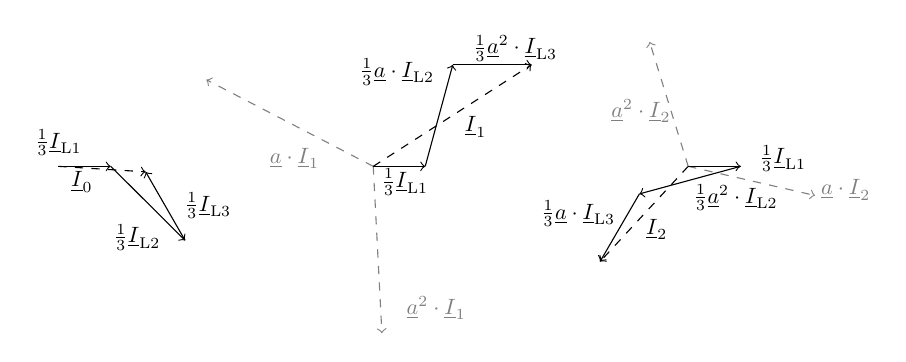
\begin{tikzpicture}
    \draw [->] [dashed] (0, -6) -- (2.01, -4.71);
    \draw [->, gray] [dashed] (0, -6) -- (-2.12, -4.9);
    \draw [->, gray] [dashed] (0, -6) -- (0.11, -8.12);
    \draw [->] (0, -6) -- (0.66, -6);
    \draw [->] (0.66, -6) -- (1.01, -4.71);
    \draw [->] (1.01, -4.71) -- (2.01, -4.71);

    \draw (1.3, -5.5) node [scale=0.8] {$\underline{I}_{\mathrm{1}}$};
    \draw (-1, -5.9) node [scale=0.8, gray] {$\underline{a}\cdot\underline{I}_{\mathrm{1}}$};
    \draw (0.8, -7.8) node [scale=0.8, gray] {$\underline{a}^2\cdot\underline{I}_{\mathrm{1}}$};
    \draw (0.4, -6.2) node [scale=0.8] {$\frac{1}{3}\underline{I}_{\mathrm{L1}}$};
    \draw (1.8, -4.5) node [scale=0.8] {$\frac{1}{3}\underline{a}^2\cdot\underline{I}_{\mathrm{L3}}$};
    \draw (0.3, -4.8) node [scale=0.8] {$\frac{1}{3}\underline{a}\cdot\underline{I}_{\mathrm{L2}}$};

    \draw [->] [dashed] (4, -6) -- (2.88, -7.21);
    \draw [->, gray] [dashed] (4, -6) -- (5.61, -6.37);
    \draw [->, gray] [dashed] (4, -6) -- (3.51, -4.42);
    \draw [->] (4, -6) -- (4.666, -6);
    \draw [->] (4.666, -6) -- (3.38, -6.35);
    \draw [->] (3.38, -6.35) -- (2.88, -7.21);

    \draw (3.6, -6.8) node [scale=0.8] {$\underline{I}_{\mathrm{2}}$};
    \draw (6, -6.3) node [scale=0.8, gray] {$\underline{a}\cdot\underline{I}_{\mathrm{2}}$};
    \draw (3.4, -5.3) node [scale=0.8, gray] {$\underline{a}^2\cdot\underline{I}_{\mathrm{2}}$};
    \draw (5.2, -5.9) node [scale=0.8] {$\frac{1}{3}\underline{I}_{\mathrm{L1}}$};
    \draw (4.6, -6.4) node [scale=0.8] {$\frac{1}{3}\underline{a}^2\cdot\underline{I}_{\mathrm{L2}}$};
    \draw (2.6, -6.6) node [scale=0.8] {$\frac{1}{3}\underline{a}\cdot\underline{I}_{\mathrm{L3}}$};

    \draw [->] [dashed] (-4, -6) -- (-2.89, -6.07);
    \draw [->] (-4, -6) -- (-3.334, -6);
    \draw [->] (-3.334, -6) -- (-2.39, -6.94);
    \draw [->] (-2.39, -6.94) -- (-2.89, -6.07);

    \draw (-3.7, -6.2) node [scale=0.8] {$\underline{I}_{\mathrm{0}}$};
    \draw (-4, -5.7) node [scale=0.8] {$\frac{1}{3}\underline{I}_{\mathrm{L1}}$};
    \draw (-3, -6.9) node [scale=0.8] {$\frac{1}{3}\underline{I}_{\mathrm{L2}}$};
    \draw (-2.1, -6.5) node [scale=0.8] {$\frac{1}{3}\underline{I}_{\mathrm{L3}}$};
\end{tikzpicture}
                  }
              \end{figure}
              
              Anmerkung: Das Erstellen der Zeigerdiagramme ist ein guter Weg um die errechneten Ergebnisse aus 3. zu überprüfen.
              Die Wege der Zeiger, die aus dem Originalsystem genommen werden, müssen da enden, wo auch der Zeiger des transformierten Systems hinführt.
              Stimmen die Endpunkte nicht überein, wurde in einer der Rechnungen ein Fehler gemacht.
              
    \end{itemize}
}
